\chapter{Introducción}

\section{Motivación}

El genoma humano presenta variaciones en pares de bases individuales que determinan la diversidad genética entre los diferentes individuos. A estas mutaciones puntuales se les denomina polimorfismos de un solo nucleótido (SNPs) \cite{hinds2005whole}. Por ejemplo, si en una cadena de ADN la mayoría de la población presenta la base de citosina (C) en una posición específica, pero una fracción presenta timina (T), dicha alteración posicional constituye un SNP (véase la Figura \ref{fig:ejemplo_snp}).

\begin{figure}[H]
    \centering
    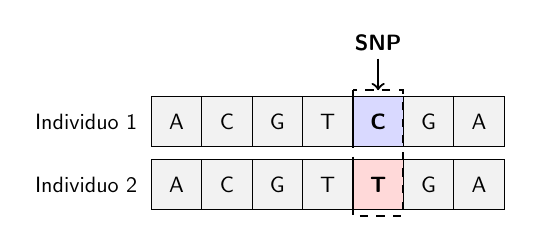
\begin{tikzpicture}[font=\sffamily, scale=0.8, transform shape]
        \tikzstyle{base}=[draw, minimum width=0.8cm, minimum height=0.8cm, fill=gray!10]
        \tikzstyle{snp1}=[draw, minimum width=0.8cm, minimum height=0.8cm, fill=blue!15]
        \tikzstyle{snp2}=[draw, minimum width=0.8cm, minimum height=0.8cm, fill=red!15]
        
        \node[left=0.5cm] at (0, 1) {Individuo 1};
        \node[base] at (0,1) {A}; \node[base] at (0.8,1) {C}; \node[base] at (1.6,1) {G}; \node[base] at (2.4,1) {T}; \node[snp1] at (3.2,1) {\textbf{C}}; \node[base] at (4.0,1) {G}; \node[base] at (4.8,1) {A};
        
        \node[left=0.5cm] at (0, 0) {Individuo 2};
        \node[base] at (0,0) {A}; \node[base] at (0.8,0) {C}; \node[base] at (1.6,0) {G}; \node[base] at (2.4,0) {T}; \node[snp2] at (3.2,0) {\textbf{T}}; \node[base] at (4.0,0) {G}; \node[base] at (4.8,0) {A};
        
        % Flecha y recuadro indicando el SNP
        \draw[->, thick] (3.2, 2.0) node[above] {\textbf{SNP}} -- (3.2, 1.5);
        \draw[dashed, thick] (2.8, 1.5) rectangle (3.6, -0.5);
    \end{tikzpicture}
    \caption[Representación visual de un Polimorfismo de un Solo Nucleótido (SNP)]{Representación visual de un Polimorfismo de un Solo Nucleótido (SNP). La variación alélica se manifiesta en una única posición de la secuencia genética, marcando la diferencia entre los individuos de la población.}
    \label{fig:ejemplo_snp}
\end{figure}

El análisis estructurado de estas secuencias tiene una relevancia médica directa, ya que constituyen la base de los Estudios de Asociación del Genoma Completo (GWAS, por sus siglas en inglés: \textit{Genome-Wide Association Studies}) para identificar predisposiciones a enfermedades complejas \cite{hinds2005whole}.

Genotipar, es decir, secuenciar y analizar de forma exhaustiva la totalidad de los millones de SNPs presentes en el genoma de un individuo, resulta prohibitivo. Este enfoque masivo implica unos altos costes económicos de laboratorio y requiere un esfuerzo de procesamiento computacional inasumible \cite{ting2010multi}. Sin embargo, debido a los fenómenos de recombinación biológica y al desequilibrio de ligamiento, los SNPs ubicados en regiones adyacentes tienden a heredarse en bloque. Esto genera una elevada redundancia de información \cite{bafna2003haplotypes}. A partir de esta propiedad biológica surge la necesidad de aplicar la selección de etiquetas SNP, un procedimiento que consiste en identificar un subconjunto mínimo de SNPs representativos capaces de capturar y distinguir la variabilidad genética global de la población \cite{ting2010multi, moqa2022assessing}. La extracción de este subconjunto reduce drásticamente la dimensionalidad de los datos, haciendo factibles y rentables los estudios genéticos a gran escala.

Sin embargo, descubrir cuál es exactamente ese subconjunto óptimo no es una tarea biológica trivial. Requiere analizar matemáticamente las intrincadas relaciones de dependencia entre miles de SNPs, lo que transforma una necesidad médica en un desafío mayúsculo de optimización e ingeniería algorítmica.

El presente Trabajo Fin de Grado aborda matemáticamente la problemática de la selección de etiquetas SNP. Su resolución presenta una importancia crítica, ya que el coste y tiempo de procesamiento de cada paciente se reduce drásticamente por cada SNP que logre ser descartado sin perder información representativa, lo que acerca la viabilidad comercial y clínica de estos paneles de diagnóstico poblacional.

\section{Complejidad del problema y reto computacional}

Desde una perspectiva analítica, la selección de etiquetas SNP se modela como un problema de optimización combinatoria estructuralmente equivalente al problema clásico de Cobertura de Conjuntos. Esta clasificación lo enmarca dentro de la categoría de problemas computacionales NP-Duro \cite{bafna2003haplotypes}. Esto implica que el tiempo de cómputo necesario para asegurar la localización de la combinación óptima crece de manera exponencial en función de la longitud de la cadena genética de entrada, descartando por completo el uso de métodos de resolución exactos. Por ejemplo, dada una secuencia empírica de apenas $1000$ SNPs, explorar por fuerza bruta todas las combinaciones posibles para extraer un panel de $50$ etiquetas SNP requeriría evaluar el coeficiente binomial $\binom{1000}{50}$, lo que equivale a más de $10^{84}$ subconjuntos distintos. Incluso si se utilizara un clúster de supercomputación capaz de procesar un billón de combinaciones por segundo, el tiempo de cálculo superaría con creces la edad del universo.

Para abordar espacios de búsqueda de tal magnitud, resulta obligatorio recurrir a técnicas heurísticas de inteligencia artificial, en concreto, a los Algoritmos Evolutivos (EAs) \cite{ting2010multi}. Además, la selección de etiquetas SNP actual no puede reducirse a minimizar únicamente el coste del panel genético (compacidad). Resulta estrictamente necesario optimizar de manera simultánea otros factores críticos: la robustez del panel frente a errores empíricos de lectura (tolerancia a fallos), la capacidad de distinción media entre secuencias (disimilitud) y la varianza equitativo de dicha distinción (balance) \cite{ting2010multi, moqa2022assessing}. Al formular el desafío matemático con estas cuatro funciones objetivo en conflicto, el problema escapa de las capacidades de los Algoritmos Evolutivos Multiobjetivo (MOEAs) clásicos \cite{ishibuchi2008evolutionary}, haciendo indispensable la aplicación de Algoritmos Evolutivos de Muchos Objetivos (MaOEAs) \cite{moqa2022assessing}. Estas arquitecturas son las únicas preparadas para sostener una presión selectiva estable y converger de manera eficiente hacia frentes de Pareto en espacios de alta dimensionalidad.

\section{Estructura de la memoria}

El presente documento queda estructurado de la siguiente manera:
\begin{itemize}
    \item El \textbf{Capítulo 2} define los objetivos generales y específicos que articulan el desarrollo del proyecto.
    \item El \textbf{Capítulo 3} revisa el estado del arte aplicado a este dominio.
    \item El \textbf{Capítulo 4} detalla el diseño metodológico, incluyendo la parametrización experimental, la formulación matemática de los objetivos y los EAs evaluados.
    \item El \textbf{Capítulo 5} analiza los resultados empíricos extraídos de las ejecuciones mediante un análisis estadístico inferencial.
    \item El \textbf{Capítulo 6} recoge las conclusiones finales derivadas del estudio y propone diferentes líneas de trabajo futuro.
\end{itemize}